\chapter{Обробка Природної Мови.}

Велика кількість даних у багатьох реальних наборах даних представлена у вигляді так званого вільного тексту (free text). Це є, наприклад, коментарі користувачів, телеметрія програмних додатків, будь-які «неструктуровані» поля, та багато чого іншого.

Обчислювальна обробка природної мови полягає в тому, що ми пишемо комп'ютерні програми, які можуть розуміти природну мову. Обробка природної мови (NLP) займається тим, як перетворити текст — часто нечіткий і непідготовлений — у форму, зручну для аналізу та моделювання. В цьому розділі ми спробуємо отримати деяку значущу інформацію з неструктурованих текстових даних.

\section{Попередня обробка тексту.}

\subsection{Очищення тексту.}

Першим кроком до роботи з такими даними зазвичай стає підготовка тексту: приведення символів до одного регістру, видалення розділових знаків і зайвих символів, очищення чисел і зведення виробленого шуму у більш стандартизований вигляд.

Застосуємо біблотеку nltk для цих цілей. 

\begin{lstlisting}
import re
import string
from nltk.corpus import stopwords
from nltk.tokenize import word_tokenize
import nltk
\end{lstlisting}

Спершу завантажимо ресурси для роботи із найпоширенішими словами в англійській мові ('the', 'is', 'and') та для роботи із пунктуацією: "stopwords" та "punkt":

\begin{lstlisting}
nltk.download('stopwords')
nltk.download('punkt')
\end{lstlisting}

Перш за все, варто розпочати роботу з текстом із того, щоб перевести всі літери в нижній регістр:

\begin{lstlisting}
text = text.lower()
\end{lstlisting}

Та видалити розділові знаки:

\begin{lstlisting}
text = text.translate(str.maketrans('', '', string.punctuation))
\end{lstlisting}

Також із тексту можна видалити числа:

\begin{lstlisting}
text = re.sub(r'\d+', '', text)
\end{lstlisting}

Та спеціальні символи:

\begin{lstlisting}
text = re.sub(r'[^a-z\s]', '', text)
\end{lstlisting}

Щоб видалити найпоширеніші в англійській мові стоп-слова:

\begin{lstlisting}
stop_words = set(stopwords.words('english'))
text = ' '.join(word for word in word_tokenize(text) if word not in stop_words)
\end{lstlisting}

Повністю очищення тексту виглядає наступним чином:

\begin{lstlisting}
import re
import string
from nltk.corpus import stopwords
from nltk.tokenize import word_tokenize
import nltk

nltk.download('stopwords')
nltk.download('punkt')

def clean_text(text):
        text = text.lower()

        text = text.translate(str.maketrans('', '', string.punctuation))

        text = re.sub(r'\d+', '', text)

        text = re.sub(r'[^a-z\s]', '', text)

        stop_words = set(stopwords.words('english'))
        text = ' '.join(word for word in word_tokenize(text) if word not in stop_words)

        return text

sample_text = "Hello! This is an example text with numbers 123 and punctuation!!!"
cleaned_text = clean_text(sample_text)
print(cleaned_text)
\end{lstlisting}

Результат:

\begin{console}
hello example text numbers punctuation
\end{console}


\subsection{Токенізація, стемінг, лематизація, нормалізація.}

Після базового очищення йде токенізація — розбиття тексту на слова або речення, що дозволяє оперувати окремими «будівельними блоками» змісту. Далі часто застосовують стемінг або лематизацію: стемінг обрізає закінчення й повертає корінь слова, іноді утворюючи несловникові форми, тоді як лематизація намагається відновити словникову форму з урахуванням контексту. Нормалізація може також включати виправлення орфографії, розгортання абревіатур і узгодження синонімів — усе задля того, щоб одна й та сама ідея не розпадалася на багато еквівалентних представлень.

Приклад токенізації:

\begin{lstlisting}
from nltk.tokenize import word_tokenize, sent_tokenize

def tokenize_text(text):
        words = word_tokenize(text)
        sentences = sent_tokenize(text)
        return words, sentences

sample_text = "Natural Language Processing (NLP) is exciting! It enables computers to understand human language."
words, sentences = tokenize_text(sample_text)
print('Words:', words)
print('Sentences:', sentences)
\end{lstlisting}

Результат:

\begin{console}
Words: ['Natural', 'Language', 'Processing', '(', 'NLP', ')', 'is', 'exciting', '!', 'It', 'enables', 'computers', 'to', 'understand', 'human', 'language', '.']
Sentences: ['Natural Language Processing (NLP) is exciting!', 'It enables computers to understand human language.']
\end{console}

Перш ніж перейти до лематизації, варто завантажити в nltk спеціальний словник для цієї потреби:

\begin{lstlisting}
nltk.download('wordnet')
\end{lstlisting}

Стемінг та лематизація:


\begin{lstlisting}
from nltk.stem import PorterStemmer, WordNetLemmatizer
from nltk.tokenize import word_tokenize
import nltk

nltk.download('wordnet')

def apply_stemming(text):
        stemmer = PorterStemmer()
        words = word_tokenize(text)
        stemmed_words = [stemmer.stem(word) for word in words]
        return stemmed_words

def apply_lemmatization(text):
        lemmatizer = WordNetLemmatizer()
        words = word_tokenize(text)
        lemmatized_words = [lemmatizer.lemmatize(word) for word in words]
        return lemmatized_words

sample_text = "The children are playing with their toys."
print('Stemmed:', apply_stemming(sample_text))
print('Lemmatized:', apply_lemmatization(sample_text))
\end{lstlisting}

Результат:

\begin{console}
Stemmed: ['the', 'children', 'are', 'play', 'with', 'their', 'toy', '.']
Lemmatized: ['The', 'child', 'are', 'playing', 'with', 'their', 'toy', '.']
\end{console}

Приклад нормалізації з використанням модуля autocorrect:

\begin{lstlisting}
from nltk.tokenize import word_tokenize
from autocorrect import Speller
import nltk

nltk.download('punkt')

def normalize_text(text):
        spell = Speller(lang='en')
        normalization_dict = {
                "u": "you",
                "ur": "your",
                "r": "are",
                "pls": "please",
                "thx": "thanks"
        }
        words = word_tokenize(text.lower())
        normalized_words = [normalization_dict.get(word, spell(word)) for word in words]
        normalized_text = ' '.join(normalized_words)
        normalized_text = normalized_text.replace('!', '').replace('.', '').strip()
        return normalized_text

sample_text = "U r the best! Pls help me with this assignment. Thx!"
print(normalize_text(sample_text))
\end{lstlisting}

Результат:

\begin{console}
you are the best  please help me with this assignment  thanks
\end{console}



\section{Чисельне представлення тексту.}

Розуміння мови є складним завданням.

Розглянемо такий текст: «Під час полювання в Африці я застрелив слона в піжамі. Як він потрапив у мою піжаму, я не знаю». Без повного бачення всього тексту тяжко зрозуміти, що саме мається на увазі, наприклад, в першому реченні.

Основна думка полягає в наступному: ми використовуємо неймовірну кількість контексту, щоб зрозуміти значення речень природної мови. Саме з розумінням цього контексту допомагають великі мовні моделі та механізм attention в трансформерній архітектурі. Але чи завжди це настільки складно, щоб вимагати застосування передових технологій обробки тексту?

Розглянемо дві рецензії на фільм:

\textit{"Barbie is a fun movie that has surprisingly plenty of \textbf{heartwarming} moments and \textbf{good} messages to offer. The set designs are \textbf{eye-catching} and on point as well. Both Margot Robbie and Ryan Gosling nailed their parts, but it is Gosling who mostly shines."}

\textit{"It didn't grab me; I didn't find it funny anywhere. It went from the most \textbf{annoying} opening to as far as one can get annoying in every second of this film. The music was \textbf{shallow}; the production design teetered on Terry Gilliam's work but without the imagination or talent, and old 1920s/1930s film backgrounds and old Three Stooges routines were very \textbf{tiring}."}

Який з них є позитивним? Ми можемо уце зрозуміти, просто глянувши на виділені слова. Часто ми можемо дуже легко визначити «загальний зміст» тексту природною мовою, навіть не розуміючи речень.

\subsection{Мішок слів.}

Після підготовки тексту його потрібно представити чисельно. Простий і часто ефективний підхід — модель «мішка слів», при якій кожен документ кодується вектором частот слів.

Генерація wordcloud (приклад збору тексту зі сторінки та візуалізації):

\begin{lstlisting}
from wordcloud import WordCloud
from bs4 import BeautifulSoup
import requests
import re

response = requests.get("https://mathmod.chnu.edu.ua/")
root = BeautifulSoup(response.content, "lxml")
wc = WordCloud(width=800, height=400).generate(re.sub(r"\s+", " ", root.text))
wc.to_image()
\end{lstlisting}

Результат:

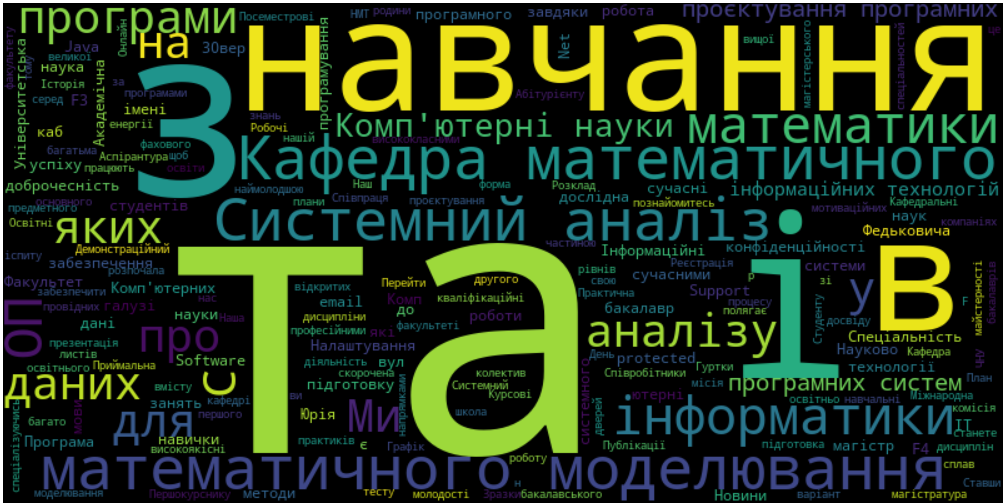
\includegraphics[scale=0.75]{img/106-1}



\subsection{TFIDF та косинусна подібність тексту.}

«Частота терміна» просто означає кількість кожного слова в документі. Позначається $tf_{i,j}$ частотою слова $i$ в документі (тексті) $j$ (іноді індекси обертаються, ми використовуємо їх для узгодженості з матрицею).

\begin{lstlisting}
documents = [
    "In Inception, the plot unfolds with thrilling action, keeping audiences on edge through a series of intense and unexpected twists.", # t_i_0 = 1
    "The story of Inception keeps audiences hooked with its thrilling action and surprising twists, making every moment unforgettable.", # t_i_1 = 1
    "The Matrix transformation preserves the vector's direction, illustrating how linear combinations affect the overall system." # t_i_2 = 0
]

document_words = [doc.lower().split() for doc in documents] 
vocab = sorted(set(sum(document_words, [])))
vocab_dict = {k:i for i,k in enumerate(vocab)}
print(vocab, "\n")
print(vocab_dict, "\n")
\end{lstlisting}

Результат:

\begin{console}
['a', 'action', 'action,', 'affect', 'and', 'audiences', 'combinations', 'direction,', 'edge', 'every', 'hooked', 'how', 'illustrating', 'in', 'inception', 'inception,', 'intense', 'its', 'keeping', 'keeps', 'linear', 'making', 'matrix', 'moment', 'of', 'on', 'overall', 'plot', 'preserves', 'series', 'story', 'surprising', 'system.', 'the', 'thrilling', 'through', 'transformation', 'twists,', 'twists.', 'unexpected', 'unfolds', 'unforgettable.', "vector's", 'with'] 

{'a': 0, 'action': 1, 'action,': 2, 'affect': 3, 'and': 4, 'audiences': 5, 'combinations': 6, 'direction,': 7, 'edge': 8, 'every': 9, 'hooked': 10, 'how': 11, 'illustrating': 12, 'in': 13, 'inception': 14, 'inception,': 15, 'intense': 16, 'its': 17, 'keeping': 18, 'keeps': 19, 'linear': 20, 'making': 21, 'matrix': 22, 'moment': 23, 'of': 24, 'on': 25, 'overall': 26, 'plot': 27, 'preserves': 28, 'series': 29, 'story': 30, 'surprising': 31, 'system.': 32, 'the': 33, 'thrilling': 34, 'through': 35, 'transformation': 36, 'twists,': 37, 'twists.': 38, 'unexpected': 39, 'unfolds': 40, 'unforgettable.': 41, "vector's": 42, 'with': 43}
\end{console}

Тепер побудуємо матрицю, яка містить кількість слів (частоту вживання термінів) для всіх документів.

\begin{lstlisting}
import numpy as np

X_tf = np.zeros((len(documents), len(vocab)), dtype=int)
for i, doc in enumerate(document_words):
    for word in doc:
        X_tf[i, vocab_dict[word]] +=1
        
print(X_tf)
\end{lstlisting}

Результат:

\begin{console}
[[1 0 1 0 1 1 0 0 1 0 0 0 0 1 0 1 1 0 1 0 0 0 0 0 1 1 0 1 0 1 0 0 0 1 1 1
  0 0 1 1 1 0 0 1]
 [0 1 0 0 1 1 0 0 0 1 1 0 0 0 1 0 0 1 0 1 0 1 0 1 1 0 0 0 0 0 1 1 0 1 1 0
  0 1 0 0 0 1 0 1]
 [0 0 0 1 0 0 1 1 0 0 0 1 1 0 0 0 0 0 0 0 1 0 1 0 0 0 1 0 1 0 0 0 1 3 0 0
  1 0 0 0 0 0 1 0]]
\end{console}


Частота вживання термінів, як правило, «перевантажена» дуже поширеними словами («the», «is», «of» тощо). 

\ding{43} Примітка: дуже поширені слова, які називаються «стоп-словами», можуть бути навіть видалені з використанням засобів nltk, як ми це обговорювали на початку цього розділа.

Ідея зворотної частоти документа полягає в тому, щоб надавати словам негативну вагу пропорційно до частоти їх вживання в усьому наборі документів.

$$idf_{i} = \log( \frac{N_{documents}}{N_{documents-with-word-i}} )$$

Як і у випадку з частотою терміна, існують також інші версії з різними масштабами, але найпоширенішим є вищезазначений логарифмічний масштаб.

Зверніть увагу, що обернена частота документа визначається лише для слів, а не для пар «слово-документ», як у випадку з частотою терміна.


\begin{lstlisting}
idf = np.log(X_tf.shape[0]/X_tf.astype(bool).sum(axis=0))
print(idf)
\end{lstlisting}

Результат:

\begin{console}
[1.09861229 1.09861229 1.09861229 1.09861229 0.40546511 0.40546511
 1.09861229 1.09861229 1.09861229 1.09861229 1.09861229 1.09861229
 1.09861229 1.09861229 1.09861229 1.09861229 1.09861229 1.09861229
 1.09861229 1.09861229 1.09861229 1.09861229 1.09861229 1.09861229
 0.40546511 1.09861229 1.09861229 1.09861229 1.09861229 1.09861229
 1.09861229 1.09861229 1.09861229 0.         0.40546511 1.09861229
 1.09861229 1.09861229 1.09861229 1.09861229 1.09861229 1.09861229
 1.09861229 0.40546511]
\end{console}


Зрештою, поєднання частоти терміна та зворотної частоти документа дає відому міру TF–IDF (term frequency inverse document frequency): 

$$tfidf_{i,j}=tf_{i,j}\times idf_{i},$$

яка підсилює рідкісні й інформативні слова й послаблює надто загальні.


\begin{lstlisting}
X_tfidf = X_tf * idf
print(X_tfidf)
\end{lstlisting}

Результат:

\begin{console}
[[1.09861229 0.         1.09861229 0.         0.40546511 0.40546511
  0.         0.         1.09861229 0.         0.         0.
  0.         1.09861229 0.         1.09861229 1.09861229 0.
  1.09861229 0.         0.         0.         0.         0.
  0.40546511 1.09861229 0.         1.09861229 0.         1.09861229
  0.         0.         0.         0.         0.40546511 1.09861229
  0.         0.         1.09861229 1.09861229 1.09861229 0.
  0.         0.40546511]
 [0.         1.09861229 0.         0.         0.40546511 0.40546511
  0.         0.         0.         1.09861229 1.09861229 0.
  0.         0.         1.09861229 0.         0.         1.09861229
  0.         1.09861229 0.         1.09861229 0.         1.09861229
  0.40546511 0.         0.         0.         0.         0.
  1.09861229 1.09861229 0.         0.         0.40546511 0.
  0.         1.09861229 0.         0.         0.         1.09861229
  0.         0.40546511]
 [0.         0.         0.         1.09861229 0.         0.
  1.09861229 1.09861229 0.         0.         0.         1.09861229
  1.09861229 0.         0.         0.         0.         0.
  0.         0.         1.09861229 0.         1.09861229 0.
  0.         0.         1.09861229 0.         1.09861229 0.
  0.         0.         1.09861229 0.         0.         0.
  1.09861229 0.         0.         0.         0.         0.
  1.09861229 0.        ]]
\end{console}


Косинусна подібність — простий спосіб виміряти схожість між двома векторними представленнями тексту: 

$$CosineSim(x,y)=\dfrac{x\cdot y}{\|x\|_{2}\|y\|_{2}}.$$

Більші числа означають, що вектори tfidf є ближчими в $n$-вимірному просторі, а отже, тексти подібніші між собою.

\begin{lstlisting}
X_tfidf_norm = X_tfidf / np.linalg.norm(X_tfidf, axis=1)[:,None]
M = X_tfidf_norm @ X_tfidf_norm.T
print(M)
\end{lstlisting}

Результат:

\begin{console}
[[1.         0.04991504 0.        ]
 [0.04991504 1.         0.        ]
 [0.         0.         1.        ]]
\end{console}

Як бачимо, тексти, що описували одні і ті ж речі, отримали більшу косинусну подібність, а третій текст з обома іншими має косинусну подібність 0.

Використання tfidf та косинусної подібності повністю:

\begin{lstlisting}
import numpy as np

documents = [
        "In Inception, the plot unfolds with thrilling action, keeping audiences on edge through a series of intense and unexpected twists.",
        "The story of Inception keeps audiences hooked with its thrilling action and surprising twists, making every moment unforgettable.",
        "The Matrix transformation preserves the vector's direction, illustrating how linear combinations affect the overall system."
]

document_words = [doc.lower().split() for doc in documents]
vocab = sorted(set(sum(document_words, [])))
vocab_dict = {k: i for i, k in enumerate(vocab)}

X_tf = np.zeros((len(documents), len(vocab)), dtype=int)
for i, doc in enumerate(document_words):
        for word in doc:
                X_tf[i, vocab_dict[word]] += 1


idf = np.log(X_tf.shape[0] / X_tf.astype(bool).sum(axis=0))
X_tfidf = X_tf * idf
X_tfidf_norm = X_tfidf / np.linalg.norm(X_tfidf, axis=1)[:, None]
M = X_tfidf_norm @ X_tfidf_norm.T
print('Cosine similarity matrix:\n', M)
\end{lstlisting}

Результат:

\begin{console}
Cosine similarity matrix:
 [[1.         0.04991504 0.        ]
 [0.04991504 1.         0.        ]
 [0.         0.         1.        ]]
\end{console}


\ding{43} Косинусна подібність добре працює для порівняння документів у просторі TF–IDF, але має й обмеження: в такому підході немає розуміння семантики слів, і різні слова, які мають близьке значення, залишаються віддаленими в просторі one‑hot або частотних векторів.

Наприклад, наступні окремі слова мають між собою відстань 1, хоча деякі із них є більш спорідненими між собою:

$$||kyiv - zhytomyr|| = ||zhytomyr - uncle|| = 1 $$



\subsection{Векторне подання слів.}

Щоб виправити недоліки косинусної подібності, використовують вбудовування слів (word embeddings) — щільні вектори фіксованого розміру, у яких семантично близькі слова займають близькі позиції у просторі. Моделі на кшталт word2vec або переднавчені матриці типу GloVe навчають векторні представлення таким чином, що арифметичні операції над векторами можуть відображати мовні відношення: наприклад, операція $\text{king} - \text{man} + \text{woman}$ зазвичай наближається до вектора, близького до $\text{queen}$. Це відкриває шлях до більш змістовних порівнянь і до знаходження синонімів, антонімів і тематичних зв'язків.

Щоб завантажити векторне подання, варто спочатку встановити модуль sentence-transformers, та завантажити претреновану трансофрмер модель:

\begin{lstlisting}
import numpy as np
from sentence_transformers import SentenceTransformer, util

model = SentenceTransformer('all-MiniLM-L6-v2')
\end{lstlisting}

Давайте глянемо, як виглядає векторне подання слова "computer" (або, хоча б, перші 10 чисел):

\begin{lstlisting}
vector = model.encode(['computer'])[0]
print('vector sample:', vector[:10])
\end{lstlisting}

Результат:

\begin{console}
vector sample: [-0.05127361  0.04783836 -0.00333908 -0.0388703  -0.03269714 -0.0328583
  0.09360427  0.03932324  0.08196709  0.01824838]
\end{console}

Тепер ми можемо обчислювати подібності між окремими словами:

\begin{lstlisting}
embeddings = model.encode(['woman', 'man', 'kyiv'])

similarity = util.cos_sim(embeddings[0], embeddings[1]).item()
print('similarity woman/man:', similarity)

similarity = util.cos_sim(embeddings[1], embeddings[2]).item()
print('similarity man/kyiv:', similarity)
\end{lstlisting}

Результат:

\begin{console}
similarity woman/man: 0.32567834854125977
similarity man/kyiv: 0.17196238040924072
\end{console}

Тепер, для прикладу, обчислимо вектор 'King - Man + Woman' та знайдемо схожі до нього.

\begin{lstlisting}
words_to_encode = ['king', 'man', 'woman']
word_vectors = model.encode(words_to_encode)

king = word_vectors[0]
man = word_vectors[1]
woman = word_vectors[2]

result_vector = king - man + woman

vocabulary = ['queen', 'princess', 'monarch', 'empress', 'man', 'computer', 'throne', 'kyiv']
vocab_embeddings = model.encode(vocabulary)

similarities = util.cos_sim(result_vector, vocab_embeddings)[0].numpy()

top_indices = np.argsort(similarities)[::-1][:5]

print('\nAnalogy results:')
for idx in top_indices:
    print(f"{vocabulary[idx]}: {similarities[idx]:.4f}")
\end{lstlisting}

Результат:

\begin{console}
Analogy results:
queen: 0.5795
monarch: 0.5469
throne: 0.4804
princess: 0.4418
empress: 0.4368
\end{console}

Як бачимо, вектор 'King - Man + Woman' доволі таки близький до вектора 'Queen'.

Проведемо тепер tfidf-аналіз та знайдемо косинусну подібність між текстами, використовуючи тепер векторне представлення кожного окремого слова.

\begin{lstlisting}
from sentence_transformers import SentenceTransformer, util

documents = [
    "kyiv has some excellent new restaurants",
    "kharkiv is a city with great cuisine",
    "postgresql is a relational database management system"
]

model = SentenceTransformer('all-MiniLM-L6-v2')

X_embeddings = model.encode(documents)
print("Embedding matrix:")
print(X_embeddings)
similarity_matrix = util.cos_sim(X_embeddings, X_embeddings)

print("\nCosinus similarity matrix:")
print(similarity_matrix.numpy())
\end{lstlisting}

Результат:

\begin{console}
Embedding matrix:
[[-0.00245756 -0.05211234  0.05479724 ...  0.05498891 -0.00664046
  -0.02283956]
 [ 0.04663361  0.06056985 -0.02163695 ...  0.04387321 -0.0416828
   0.0089187 ]
 [ 0.01276393 -0.00399948 -0.08929092 ... -0.02673415  0.04939254
   0.0399594 ]]

Cosinus similarity matrix:
[[ 1.          0.53684413 -0.01055246]
 [ 0.53684413  1.          0.03759826]
 [-0.01055246  0.03759826  1.        ]]
\end{console}


Далі стоять мовні моделі, які намагаються оцінити ймовірність слова, враховуючи контекст: $P(word_{i}\mid word_{1},\dots,word_{i-1})$. Простий, але корисний клас таких моделей — n‑грами, що враховують обмежений контекст попередніх $n-1$ слів; їх можна вважати аппроксимацією повної ймовірнісної моделі мови. Сучасні нейронні та трансформерні моделі значно перевершують n‑грами за здатністю захоплювати довготривалі залежності та контекст.

У практиці науковця з даних частина роботи полягає в доборі правильного представлення залежно від задачі: для швидкої класифікації рецензій часто достатньо TF–IDF і лінійних моделей; для складних завдань семантичного пошуку або витягнення сутностей корисні вбудовування слів і контекстні мовні моделі. Важливо пам'ятати, що підготовка даних і прості методи іноді дають вражаючі результати, і вибір інструменту має базуватись на доступності даних, вимогах до точності й обмеженнях по часу на навчання.



\ding{46} \textbf{Питання для самоконтролю.}

\begin{enumerate}
\item Що таке обробка природної мови (Natural Language Processing, NLP)?
\item Які задачі належать до сфери обробки природної мови?
\item Чому текстові дані потребують попередньої обробки?
\item Які основні етапи попередньої обробки тексту?
\item Що таке токенізація?
\item Які існують способи токенізації тексту?
\item Для чого виконується очищення тексту?
\item Які символи зазвичай видаляють під час очищення тексту?
\item Що таке стоп-слова?
\item Чому стоп-слова часто вилучають із тексту?
\item У яких випадках видаляти стоп-слова недоцільно?
\item Що таке нормалізація тексту?
\item Для чого текст переводять до нижнього регістру?
\item Чим нормалізація відрізняється від токенізації?
\item Що таке стемінг?
\item Які задачі вирішує стемінг?
\item Які переваги та недоліки стемінгу?
\item Що таке лематизація?
\item Чим лематизація відрізняється від стемінгу?
\item У яких випадках доцільніше використовувати лематизацію?
\item Що таке хмара слів (Word Cloud)?
\item Для чого використовується хмара слів?
\item Які обмеження має хмара слів як інструмент аналізу?
\item Що таке модель «мішок слів» (Bag of Words)?
\item Як формується матриця Bag of Words?
\item Які недоліки моделі Bag of Words?
\item Що таке TF (Term Frequency)?
\item Як обчислюється TF?
\item Що таке IDF (Inverse Document Frequency)?
\item Чому рідкісні слова мають вищу вагу в IDF?
\item Що таке TF-IDF?
\item Які переваги TF-IDF порівняно з Bag of Words?
\item У яких задачах застосовується TF-IDF?
\item Що таке векторне подання тексту?
\item Як текст перетворюється на числовий вектор?
\item Що таке косинусна подібність?
\item Як інтерпретується значення косинусної подібності?
\item Чому косинусна подібність є популярною мірою схожості документів?
\item Що таке векторне подання слів (Word Embeddings)?
\item Чим векторні подання слів відрізняються від TF-IDF?
\item Які переваги мають моделі Word2Vec та GloVe?
\item Які сучасні моделі контекстних векторних подань слів існують?
\item У яких задачах використовуються векторні подання слів?
\item Які бібліотеки Python найчастіше застосовують для обробки природної мови?
\item Які сучасні напрями розвитку технологій обробки природної мови пов'язані з великими мовними моделями (LLM)?
\end{enumerate}